\documentclass[6pt,letterpaper]{article}
\usepackage[margin=0.25in, top=0.3in, bottom=0.25in]{geometry}
\usepackage{amsmath,amssymb}
\usepackage{multicol}
\usepackage{xcolor}
\usepackage{mdframed}
\usepackage[expansion=false]{microtype}
\usepackage{fancyhdr}
\usepackage{booktabs}
\usepackage{colortbl}
\usepackage{array}
\usepackage{graphicx}

% Colors (match Midterm 1 sheet for visual consistency)
\definecolor{purple}{HTML}{534AB7}\definecolor{purplebg}{HTML}{EEEDFE}
\definecolor{teal}{HTML}{0F6E56}\definecolor{tealbg}{HTML}{E1F5EE}
\definecolor{coral}{HTML}{993C1D}\definecolor{coralbg}{HTML}{FAECE7}
\definecolor{amber}{HTML}{854F0B}\definecolor{amberbg}{HTML}{FAEEDA}
\definecolor{green}{HTML}{3B6D11}\definecolor{greenbg}{HTML}{EAF3DE}
\definecolor{blue}{HTML}{0C447C}\definecolor{bluebg}{HTML}{E6F1FB}
\definecolor{gray}{HTML}{444441}\definecolor{graybg}{HTML}{F1EFE8}
\definecolor{pink}{HTML}{72243E}\definecolor{pinkbg}{HTML}{FBEAF0}
\definecolor{rowB}{HTML}{F2F2EF}

\newmdenv[linewidth=0.4pt,innerleftmargin=3pt,innerrightmargin=3pt,
  innertopmargin=2pt,innerbottommargin=2pt,skipabove=1pt,skipbelow=1pt]{ebox}

\newcommand{\shead}[3]{%
  \noindent\colorbox{#1}{\parbox{\dimexpr\linewidth-2\fboxsep\relax}%
  {\color{#2}\bfseries\fontsize{6}{7}\selectfont #3}}\vspace{0.5pt}}

\newcommand{\eq}[2]{\noindent{\color{gray}\bfseries\fontsize{5.8}{6}\selectfont#1}\enspace{\color{teal}\fontsize{5.5}{6}\selectfont\textit{#2}}}

\setlength{\parindent}{0pt}\setlength{\parskip}{0pt}
\setlength{\columnsep}{5pt}\setlength{\multicolsep}{1pt}

\pagestyle{fancy}\fancyhf{}
\renewcommand{\headrulewidth}{0.3pt}
\fancyhead[L]{\fontsize{6.5}{7}\selectfont\textbf{ECE332 --- Final Cheat Sheet (HW3 + HW4)}}
\fancyhead[R]{\fontsize{6.5}{7}\selectfont Bao Nguyen}

\graphicspath{{../img/}{../../Cheatsheets/Exam1/img/}{../../../Textbook/tables/}}

\begin{document}

%%=============================================================
%% PAGE 1 --- HW3 (BOUNDARIES + WAVEGUIDES)
%%=============================================================
\fontsize{6}{7.5}\selectfont
\setlength{\abovedisplayskip}{1pt}\setlength{\belowdisplayskip}{1.5pt}
\setlength{\abovedisplayshortskip}{0pt}\setlength{\belowdisplayshortskip}{0pt}
\begin{multicols}{3}

%-- Column 1 -----------------------------------
\shead{purplebg}{purple}{$\tilde{\mathbf{E}}$ PHASOR TEMPLATES (Air: $\varepsilon_r\!=\!\mu_r\!=\!1$)}
\begin{ebox}
\eq{Wavenumber per medium}{nonmag.}
\[k_i = \tfrac{\omega\sqrt{\varepsilon_{r,i}}}{c}\;(\text{rad/m})\quad\Rightarrow\;k_2 = k_1\sqrt{\varepsilon_{r,2}/\varepsilon_{r,1}}\]

\eq{Direction table}{$u\in\{x,y,z\}$ = axis perp.\ to boundary}\\[1pt]
{\centering\makebox[0.98\linewidth][c]{{\setlength{\tabcolsep}{3pt}\begin{tabular}{@{}cccc@{}}
\toprule
Inc dir & Inc & Refl & Trans\\
\midrule
\rowcolor{rowB}$+\hat{u}$ & $e^{-jk_1u}$ & $e^{+jk_1u}$ & $e^{-jk_2u}$\\
$-\hat{u}$ & $e^{+jk_1u}$ & $e^{-jk_1u}$ & $e^{+jk_2u}$\\
\bottomrule
\end{tabular}}}\par}
\textit{$+\hat{u}$ direction $\Leftrightarrow$ Med 2 at $u\!\ge\!0$. Reflected sign flips, transmitted matches incident.}\\[2pt]

\textit{General template (incident has pol.\ $\hat{e}$, amplitude $a_0$):}
\[\begin{aligned}
\tilde{\mathbf{E}}^i &= a_0\hat{e}\,e^{\mp jk_1u}\;\text{(V/m)}&&\text{\tiny (incident wave, Med 1)}\\
\tilde{\mathbf{E}}^r &= \Gamma\,a_0\hat{e}\,e^{\pm jk_1u}\;\text{(V/m)}&&\text{\tiny (reflected wave, Med 1)}\\
\tilde{\mathbf{E}}^t &= \tau\,a_0\hat{e}\,e^{\mp jk_2u}\;\text{(V/m)}&&\text{\tiny (transmitted wave, Med 2)}
\end{aligned}\]
\textit{(lossy med 2: replace $e^{\mp jk_2u}$ with $e^{\mp\alpha_2 u}e^{\mp j\beta_2 u}$)}\\[1pt]
\textit{Total in medium 1: $\tilde{\mathbf{E}}_1 = \tilde{\mathbf{E}}^i + \tilde{\mathbf{E}}^r$.}\\[1pt]
\eq{$\hat{e}$ by polarization}{plug into templates above}
{\centering\makebox[0.98\linewidth][c]{{\setlength{\tabcolsep}{2pt}\begin{tabular}{@{}p{0.30\linewidth}p{0.34\linewidth}p{0.30\linewidth}@{}}
\toprule
Pol. & $\hat{e}$ & Note\\
\midrule
\rowcolor{rowB}Lin.\ $\hat{x}$ & $\hat{x}$ & $E_y=0$\\
Lin.\ $\hat{y}$ & $\hat{y}$ & $E_x=0$\\
\rowcolor{rowB}Lin.\ at $45^\circ$ & $(\hat{x}+\hat{y})/\sqrt{2}$ & in phase\\
RHC & $\hat{x}-j\hat{y}$ & $\delta=-\pi/2$\\
\rowcolor{rowB}LHC & $\hat{x}+j\hat{y}$ & $\delta=+\pi/2$\\
General & $a_x\hat{x}+a_y e^{j\delta}\hat{y}$ & elliptical\\
\bottomrule
\end{tabular}}}\par}
\textit{\color{coral}$\Gamma, \tau$ act on $\hat{e}$ unchanged. Only swap the polarization, not the formulas.}
\end{ebox}

\vspace{2pt}
\shead{bluebg}{blue}{TABLE 8-2 --- $\Gamma, \tau, R, T$ SUMMARY}
\begin{ebox}
\textit{\color{coral}\textbf{Med.\ 1} ($z<0$) incident side; \textbf{Med.\ 2} ($z\ge0$) transmitted.}\\[1pt]
{\centering\makebox[0.98\linewidth][c]{{\setlength{\tabcolsep}{0.5pt}\fontsize{4.6}{5.4}\selectfont\begin{tabular}{@{}p{0.205\linewidth}|p{0.13\linewidth}|p{0.32\linewidth}|p{0.325\linewidth}@{}}
\toprule
 & \textbf{Normal} ($\theta_i\!=\!0$) & $\boldsymbol{\perp}$ \textbf{pol} & $\boldsymbol{\parallel}$ \textbf{pol}\\
\midrule
\rowcolor{rowB}$\Gamma$ \tiny refl.\ wav & $\tfrac{\eta_2-\eta_1}{\eta_2+\eta_1}$ & $\tfrac{\eta_2\cos\theta_i-\eta_1\cos\theta_t}{\eta_2\cos\theta_i+\eta_1\cos\theta_t}$ & $\tfrac{\eta_2\cos\theta_t-\eta_1\cos\theta_i}{\eta_2\cos\theta_t+\eta_1\cos\theta_i}$\\
$\tau$ \tiny trans.\ wav & $\tfrac{2\eta_2}{\eta_2+\eta_1}$ & $\tfrac{2\eta_2\cos\theta_i}{\eta_2\cos\theta_i+\eta_1\cos\theta_t}$ & $\tfrac{2\eta_2\cos\theta_i}{\eta_2\cos\theta_t+\eta_1\cos\theta_i}$\\
\rowcolor{rowB}$\tau$ rel.\ & $\tau\!=\!1\!+\!\Gamma$ & $\tau_\perp\!=\!1\!+\!\Gamma_\perp$ & $\tau_\parallel\!=\!(1\!+\!\Gamma_\parallel)\tfrac{\cos\theta_i}{\cos\theta_t}$\\
$R$ \tiny refl.\ pwr & $|\Gamma|^2$ & $|\Gamma_\perp|^2$ & $|\Gamma_\parallel|^2$\\
\rowcolor{rowB}$T$ \tiny trans.\ pwr & $|\tau|^2\tfrac{\eta_1}{\eta_2}$ & $|\tau_\perp|^2\tfrac{\eta_1\cos\theta_t}{\eta_2\cos\theta_i}$ & $|\tau_\parallel|^2\tfrac{\eta_1\cos\theta_t}{\eta_2\cos\theta_i}$\\
$R\!+\!T$ \tiny total & $T\!=\!1\!-\!R$ & $T_\perp\!=\!1\!-\!R_\perp$ & $T_\parallel\!=\!1\!-\!R_\parallel$\\
\bottomrule
\end{tabular}}}\par}
\textit{\color{blue}Notes: $\sin\theta_t\!=\!\sqrt{\mu_1\varepsilon_1/\mu_2\varepsilon_2}\sin\theta_i$;\ nonmag.\ $\Rightarrow\eta_2/\eta_1\!=\!n_1/n_2$.}\\[2pt]

\eq{Intrinsic impedance $\eta_i$}{plug into table above}
\[\eta_i = \sqrt{\tfrac{\mu_r}{\varepsilon_r}}\,\eta_0 \xrightarrow{\mu_r=1} \tfrac{\eta_0}{\sqrt{\varepsilon_{r,i}}}\;(\Omega)\qquad \eta_0=120\pi\!\approx\!377\,\Omega\]
\textit{\color{coral}Default $\mu_r=1$ (air, dielectric). Use $\mu_r\!\ne\!1$ only if problem says ``ferromagnetic''/iron/ferrite/etc.}

\eq{Low-loss correction $\eta_c$}{$\sigma/(\omega\varepsilon)\ll1$}
\[\eta_c \approx \sqrt{\tfrac{\mu}{\varepsilon'}}\!\left(1+j\tfrac{\sigma}{2\omega\varepsilon'}\right) \xrightarrow{\text{drop }j}\; \tfrac{\eta_0}{\sqrt{\varepsilon_r}}\]
\textit{\color{coral}For $\Gamma$/$\tau$ just use $\eta_0/\sqrt{\varepsilon_r}$. The $j$ term is for $|\eta_c|, \theta_\eta$. See LOSSY MEDIA --- 5 CASES for all regimes.}
\end{ebox}

\vspace{2pt}
\shead{coralbg}{coral}{POWER REFLECTION \& TRANSMISSION}
\begin{ebox}
\eq{\% reflected}{always}
\[\%P_r = 100\,|\Gamma|^2\]
\eq{\% transmitted}{$\eta$-ratio matters!}
\[\%P_t = 100\,|\tau|^2\,\frac{\eta_1}{\eta_2}\]
\textit{Check: $\%P_r + \%P_t = 100$.}
\end{ebox}

\columnbreak

%-- Column 2 -----------------------------------
\shead{tealbg}{teal}{SNELL'S LAW --- OBLIQUE INCIDENCE}
\begin{ebox}
\eq{Single boundary}{angles from normal}
\[\sin\theta_2 = \sin\theta_1\sqrt{\tfrac{\varepsilon_{r1}}{\varepsilon_{r2}}} = \sin\theta_1\,\tfrac{n_1}{n_2}\]

\eq{Multilayer chain}{stack of slabs $1\to2\to3\to4$}
\[\sin\theta_{i+1} = \sin\theta_i\sqrt{\tfrac{\varepsilon_{r,i}}{\varepsilon_{r,i+1}}}\]

\eq{Air--slabs--air shortcut}{outer media identical}
\[\theta_{\text{exit}} = \theta_{\text{incident}}\]
\textit{\color{coral}Snell only sets angles. Reflection/transmission \emph{magnitudes} need Fresnel coefficients (parallel vs perpendicular).}
\end{ebox}

\vspace{2pt}
\shead{tealbg}{teal}{LATERAL DISPLACEMENT}
\begin{ebox}
\begin{center}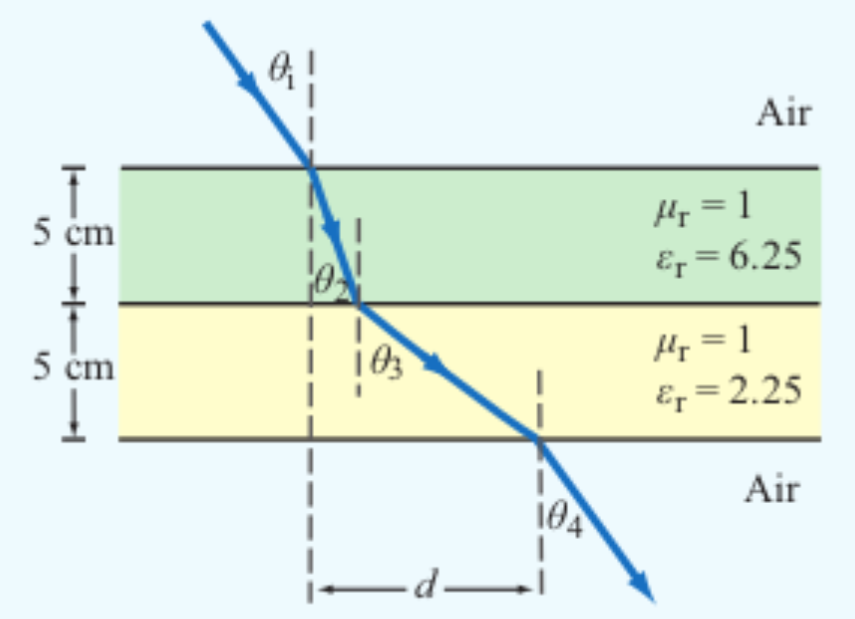
\includegraphics[width=0.65\linewidth]{p3_layered_diagram}\end{center}
\eq{Beam offset through $N$ slabs}{thickness $t_i$, refracted angle inside slab $i$}

\eq{Slab-indexed}{$\theta_i = $ angle inside slab $i$;\ $t_i = $ slab thickness (m)}
\[d = \sum_{i=1}^{N} t_i\,\tan\theta_i\]
\textit{The angle ($\theta_i$) in the formula is always the one the ray makes \emph{inside that slab of height ($t_i$)}.}
\end{ebox}

\vspace{2pt}
\shead{coralbg}{coral}{LOSSY MEDIA --- 5 CASES}
\begin{ebox}
\eq{Loss tangent}{$\varepsilon'\!=\!\varepsilon_r\varepsilon_0$;\, $\varepsilon_0\!=\!8.854\!\times\!10^{-12}$ F/m}
\[\tfrac{\varepsilon''}{\varepsilon'} = \tfrac{\sigma}{\omega\varepsilon_r\varepsilon_0}\]

{\centering\makebox[0.98\linewidth][c]{{\setlength{\tabcolsep}{2pt}\fontsize{5.6}{6.5}\selectfont\begin{tabular}{@{}p{0.28\linewidth}p{0.22\linewidth}p{0.43\linewidth}@{}}
\toprule
Type & $\sigma/\omega\varepsilon$ & $\eta_c,\;\alpha,\;\beta$\\
\midrule
\rowcolor{rowB}Lossless ($\sigma\!=\!0$) & 0 & $\eta\!=\!\eta_0/\sqrt{\varepsilon_r}$ exact\newline $\alpha\!=\!0$,\;$\beta\!=\!\omega\sqrt{\varepsilon_r}/c$\\
Low-loss & $<10^{-2}$ & $\eta_c\!\approx\!\tfrac{\eta_0}{\sqrt{\varepsilon_r}}\!\left(1{+}j\tfrac{\sigma}{2\omega\varepsilon'}\right)$\newline $\alpha\!\approx\!\tfrac{\sigma\eta_0}{2\sqrt{\varepsilon_r}}$,\;$\beta\!\approx\!\tfrac{\omega\sqrt{\varepsilon_r}}{c}$\\
\rowcolor{rowB}Quasi-cond. & $10^{-2}$--$10^2$ & exact: $(\eta/\sqrt{X})e^{j\theta_\eta}$\newline see below\\
Good cond. & $>10^2$ & $\eta_c\!\approx\!(1{+}j)\sqrt{\pi f\mu/\sigma}$\newline $\alpha\!\approx\!\beta\!\approx\!\sqrt{\pi f\mu\sigma}$\\
\rowcolor{rowB}Magnetic & any & keep full $\sqrt{\mu_r/\varepsilon_r}\,\eta_0$\\
\bottomrule
\end{tabular}}}\par}
\textit{\color{coral}For $\Gamma/\tau$: drop $j$ correction; use $\eta_0/\sqrt{\varepsilon_r}$. Magnetic: keep $\mu_r$.}

\eq{Low-loss quick params}{$\sigma/(\omega\varepsilon)\!\ll\!1$, $\mu_r\!=\!1$}
\[\alpha\!\approx\!\tfrac{\sigma\eta_0}{2\sqrt{\varepsilon_r}}\,\text{(Np/m)},\;\beta\!\approx\!\tfrac{\omega\sqrt{\varepsilon_r}}{c}\,\text{(rad/m)},\;\eta_c\!\approx\!\tfrac{\eta_0}{\sqrt{\varepsilon_r}}\,(\Omega)\]

\eq{Exact (quasi-cond)}{$X=\sqrt{1+(\varepsilon''/\varepsilon')^2}$}
\[\alpha=\omega\sqrt{\tfrac{\mu\varepsilon'}{2}}\sqrt{X{-}1},\;\;\beta=\omega\sqrt{\tfrac{\mu\varepsilon'}{2}}\sqrt{X{+}1}\]
\[\theta_\eta = \tfrac{1}{2}\arctan\!\tfrac{\sigma}{\omega\varepsilon'}\]
\end{ebox}

\columnbreak

%-- Column 3 -----------------------------------
\shead{coralbg}{coral}{RECTANGULAR WAVEGUIDE --- MODES}
\begin{ebox}
\eq{TE mode}{$E_z=0$, $H_z\ne0$}\\
\eq{TM mode}{$H_z=0$, $E_z\ne0$}\\[1pt]
\textit{Dimensions $a\times b$ with $a>b$ along $\hat{x},\hat{y}$; wave in $\hat{z}$.}\\[1pt]
\eq{$E_x$ form (TE)}{read $m,n$ from arguments}
\[E_x \propto \cos\!\left(\tfrac{m\pi x}{a}\right)\sin\!\left(\tfrac{n\pi y}{b}\right)\sin(\omega t-\beta z)\]
\textit{coef. on $x$ = $m\pi/a$; coef. on $y$ = $n\pi/b$.}\\[1pt]

\eq{Identify TE$_{mn}$ vs TM$_{mn}$}{cos/sin pattern of $E_x$ is identical for both!}\\
1.\ Read the problem statement (e.g.\ ``a TE wave''~$\to$ TE).\\
2.\ If $m\!=\!0$ or $n\!=\!0$ in the mode label\ $\Rightarrow$ must be TE (TM forbids 0).\\
3.\ Source field $H_z(x,y)$ given $\Rightarrow$ TE.\ Source field $E_z(x,y)$ given $\Rightarrow$ TM.\\[1pt]
\textit{\color{coral}TE allows at least one of $m,n\!\ge\!1$ (other can be 0). TM needs both $m,n\!\ge\!1$. That's why TE$_{10}$ exists but TM$_{10}$ doesn't.}
\end{ebox}

\vspace{2pt}
\shead{coralbg}{coral}{TABLE 8-3 --- FULL FIELD COMPONENTS}
\begin{ebox}
\textit{All fields carry an $e^{-j\beta z}$ factor (omitted below). $k_c^2 = (m\pi/a)^2+(n\pi/b)^2$.}\\[1pt]

\eq{TE mode}{generator: $\tilde{H}_z$}
\[\tilde{H}_z = H_0\cos\!\tfrac{m\pi x}{a}\cos\!\tfrac{n\pi y}{b}\]
\[\tilde{E}_x = \tfrac{j\omega\mu}{k_c^2}\!\left(\tfrac{n\pi}{b}\right) H_0\cos\!\tfrac{m\pi x}{a}\sin\!\tfrac{n\pi y}{b}\]
\[\tilde{E}_y = -\tfrac{j\omega\mu}{k_c^2}\!\left(\tfrac{m\pi}{a}\right) H_0\sin\!\tfrac{m\pi x}{a}\cos\!\tfrac{n\pi y}{b}\]
\[\tilde{E}_z = 0,\quad \tilde{H}_x = -\tilde{E}_y/Z_\text{TE},\quad \tilde{H}_y = \tilde{E}_x/Z_\text{TE}\]

\eq{TM mode}{generator: $\tilde{E}_z$}
\[\tilde{E}_z = E_0\sin\!\tfrac{m\pi x}{a}\sin\!\tfrac{n\pi y}{b}\]
\[\tilde{E}_x = -\tfrac{j\beta}{k_c^2}\!\left(\tfrac{m\pi}{a}\right) E_0\cos\!\tfrac{m\pi x}{a}\sin\!\tfrac{n\pi y}{b}\]
\[\tilde{E}_y = -\tfrac{j\beta}{k_c^2}\!\left(\tfrac{n\pi}{b}\right) E_0\sin\!\tfrac{m\pi x}{a}\cos\!\tfrac{n\pi y}{b}\]
\[\tilde{H}_z = 0,\quad \tilde{H}_x = -\tilde{E}_y/Z_\text{TM},\quad \tilde{H}_y = \tilde{E}_x/Z_\text{TM}\]

\textit{\color{coral}TEM (plane wave) for reference: $\tilde{E}_x\!=\!E_0e^{-j\beta z}$, $\tilde{H}_y\!=\!\tilde{E}_x/\eta$, $f_c$ N/A, $k\!=\!\omega\sqrt{\mu\varepsilon}$.}
\end{ebox}

\vspace{2pt}
\shead{coralbg}{coral}{CUTOFF FREQUENCY}
\begin{ebox}
\eq{$f_{mn}$ (a.k.a.\ $f_c$ for that mode)}{$m,n$ integers $\ge0$ (not both zero)}
\[f_c \equiv f_{mn} = \tfrac{u_{p0}}{2}\sqrt{\!\left(\tfrac{m}{a}\right)^{\!2}\!+\!\left(\tfrac{n}{b}\right)^{\!2}}\;\text{(Hz)}\]

\eq{Common cutoffs ($a>b$)}{}\\
{\centering\makebox[0.98\linewidth][c]{{\setlength{\tabcolsep}{2pt}\begin{tabular}{@{}p{0.22\linewidth}p{0.70\linewidth}@{}}
\toprule
Mode & $f_{mn}$\\
\midrule
\rowcolor{rowB}$u_{p0}$ & $c/\sqrt{\varepsilon_r}$ (hollow: $u_{p0}=c$)\\
TE$_{10}$ & $f_{10}=u_{p0}/(2a)$ (dominant)\\
\rowcolor{rowB}TE$_{01}$ & $f_{01}=u_{p0}/(2b)$\\
TE$_{20}$ & $f_{20}=u_{p0}/a = 2f_{10}$\\
\rowcolor{rowB}TE$_{11}$,TM$_{11}$ & $f_{11}=\tfrac{u_{p0}}{2}\sqrt{1/a^2+1/b^2}$\\
\bottomrule
\end{tabular}}}\par}
\textit{Propagation requires $f>f_{mn}$. In $Z_\text{TE}$/$Z_\text{TM}$ and $u_g$, $f_c=f_{mn}$ of the excited mode.}
\end{ebox}

\vspace{2pt}
\shead{coralbg}{coral}{$\varepsilon_r$ FROM DISPERSION}
\begin{ebox}
\eq{Given $\omega$, $\beta$, mode $(m,n)$}{result is unitless}
\[\varepsilon_r = \tfrac{c^2}{\omega^2}\!\left[\beta^2 + \!\left(\tfrac{m\pi}{a}\right)^{\!2}\!+\!\left(\tfrac{n\pi}{b}\right)^{\!2}\right]\;(\text{unitless})\]
\textit{Inputs: $\omega$ (rad/s), $\beta$ (rad/m), $a,b$ (m), $c=3\!\times\!10^8$ (m/s), $m,n$ (unitless).}
\end{ebox}

\vspace{2pt}
\shead{coralbg}{coral}{WAVE IMPEDANCE \& $H_y$}
\begin{ebox}
\[Z_{\text{TE}} = \tfrac{\eta}{\sqrt{1-(f_c/f)^2}}\,(\Omega)\qquad Z_{\text{TM}} = \eta\sqrt{1-(f_c/f)^2}\]
\[\eta = \tfrac{\eta_0}{\sqrt{\varepsilon_r}} \qquad H_y = \tfrac{E_x}{Z_{\text{TE}}}\;\text{(TE mode)}\]
\textit{$Z_{\text{TE}}>\eta$ always (denominator $<1$); $Z_{\text{TM}}<\eta$.}
\end{ebox}

\vspace{2pt}
\shead{amberbg}{amber}{GROUP VELOCITY \& TRAVEL TIME}
\begin{ebox}
\[u_g = u_{p0}\sqrt{1-(f_{mn}/f)^2}\;\text{(m/s)}\]
\[u_p = \tfrac{u_{p0}}{\sqrt{1-(f_{mn}/f)^2}}\;\text{(m/s)}\quad\Rightarrow\quad u_pu_g = u_{p0}^2\;\text{(m}^2\text{/s}^2)\]
\[t = L/u_g\;\text{(s)}\quad\text{travel time through guide of length }L\]
\textit{Higher modes have lower $u_g$ $\Rightarrow$ they arrive later. Group delay spread = sum over excited modes.}
\end{ebox}

\end{multicols}

% Bottom strip page 1
\vfill
\vspace{2pt}
\noindent
\begin{minipage}[t]{0.19\linewidth}
\shead{purplebg}{purple}{BOUNDARY}
\begin{ebox}
$\eta_1,\eta_2$ --- imp.\ ($\Omega$)\\
$\Gamma,\tau,R,T$ --- coeffs (unitless)\\
$\tau\!=\!1\!+\!\Gamma$;\ $R\!=\!|\Gamma|^2$\\
$k_i\!=\!\omega\sqrt{\varepsilon_{r,i}}/c$ (rad/m)\\
$\alpha_2$ (Np/m), $\beta_2$ (rad/m): lossy\\
$z\!=\!0$ --- boundary plane (m)\\
$\eta_0\!=\!120\pi\!\approx\!377\,\Omega$
\end{ebox}
\end{minipage}\hfill
\begin{minipage}[t]{0.19\linewidth}
\shead{tealbg}{teal}{SNELL / OBLIQUE}
\begin{ebox}
$\theta_i,\theta_t$ --- angles from normal\\
$n_i=\sqrt{\varepsilon_{r,i}}$ --- index of refr.\\
$t_i$ --- slab thickness (m)\\
$d$ --- lateral disp.\ (m)\\
plane of inc.\ = plane of $\hat{k}$+normal\\
$\perp$: $\mathbf{E}\perp$ this plane\\
$\parallel$: $\mathbf{E}\parallel$ this plane
\end{ebox}
\end{minipage}\hfill
\begin{minipage}[t]{0.19\linewidth}
\shead{coralbg}{coral}{WAVEGUIDE}
\begin{ebox}
$a,b$ --- wide, narrow dim.\ (m); $a>b$\\
$m,n$ --- mode indices (int.)\\
$f_{mn}$ --- cutoff (Hz)\\
$\beta$ --- prop.\ const (rad/m)\\
$Z_{\text{TE/TM}}$ --- wave imp.\ ($\Omega$)\\
$E_x,H_y$ --- field comps (V/m, A/m)\\
$\eta=\eta_0/\sqrt{\varepsilon_r}$
\end{ebox}
\end{minipage}\hfill
\begin{minipage}[t]{0.19\linewidth}
\shead{amberbg}{amber}{VELOCITIES}
\begin{ebox}
$u_{p0}=c/\sqrt{\varepsilon_r}$ --- bulk phase vel.\\
$u_p=u_{p0}/\sqrt{1-(f_c/f)^2}$\\
$u_g=u_{p0}\sqrt{1-(f_c/f)^2}$\\
$u_p u_g = u_{p0}^2$\\
$t=L/u_g$ --- travel time\\
$c=3\times10^8$ m/s
\end{ebox}
\end{minipage}\hfill
\begin{minipage}[t]{0.19\linewidth}
\shead{graybg}{gray}{POWER \& UNITS}
\begin{ebox}
$\%P_r=100|\Gamma|^2$\\
$\%P_t=100|\tau|^2\eta_1/\eta_2$\\
$\%P_r+\%P_t=100$\\
$\sigma$ (S/m), $\varepsilon$ (F/m), $\mu$ (H/m)\\
$\varepsilon_0=8.85\!\times\!10^{-12}$ F/m\\
$\mu_0=4\pi\!\times\!10^{-7}$ H/m\\
$1/(36\pi)\!\times\!10^{-9}\!\approx\!\varepsilon_0$
\end{ebox}
\end{minipage}


\end{document}
